% Figure 5.1 — CNN ASR curves, test fixed at 2000 sets, three training sizes.
\begin{figure}[p]
  \centering
  \begin{subfigure}{0.66\textwidth}
    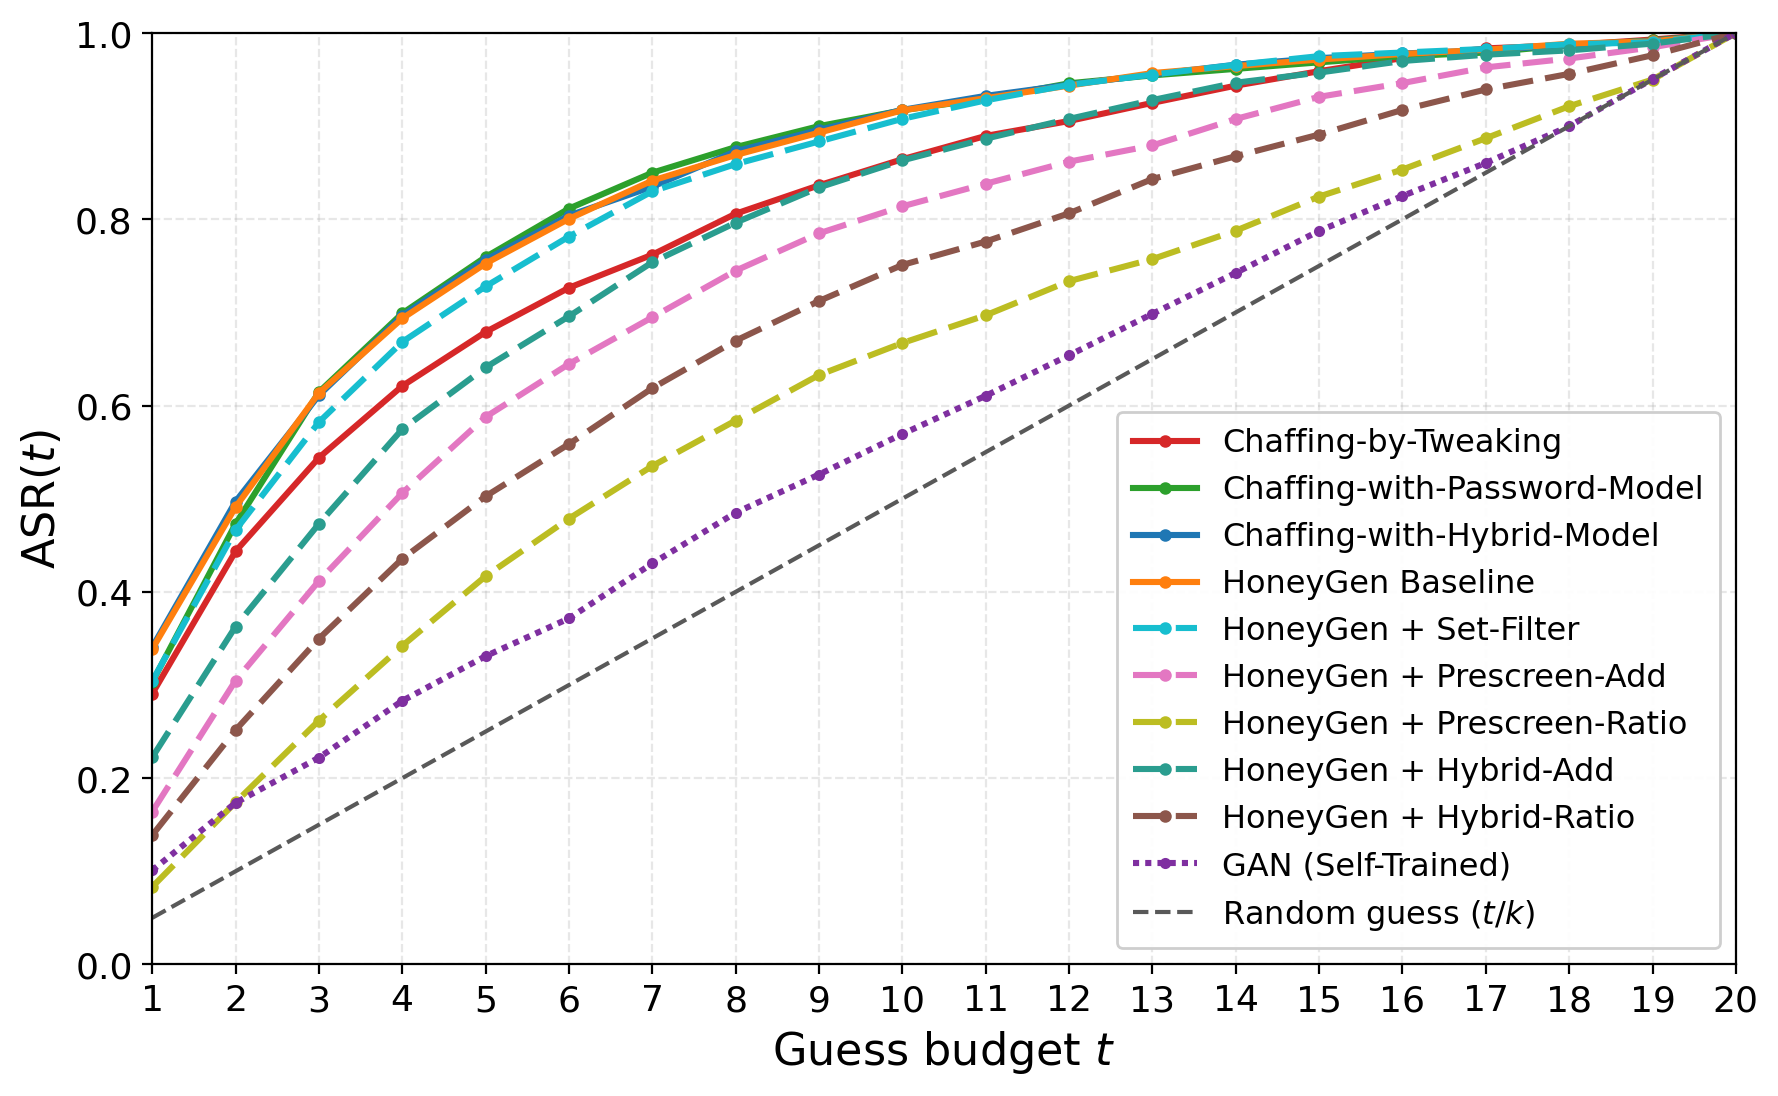
\includegraphics[width=\linewidth]{figures/cnn_N2000_e2000.png}
    \caption{$N_{\text{train}} = 2000$.}
  \end{subfigure}

  \medskip
  \begin{subfigure}{0.66\textwidth}
    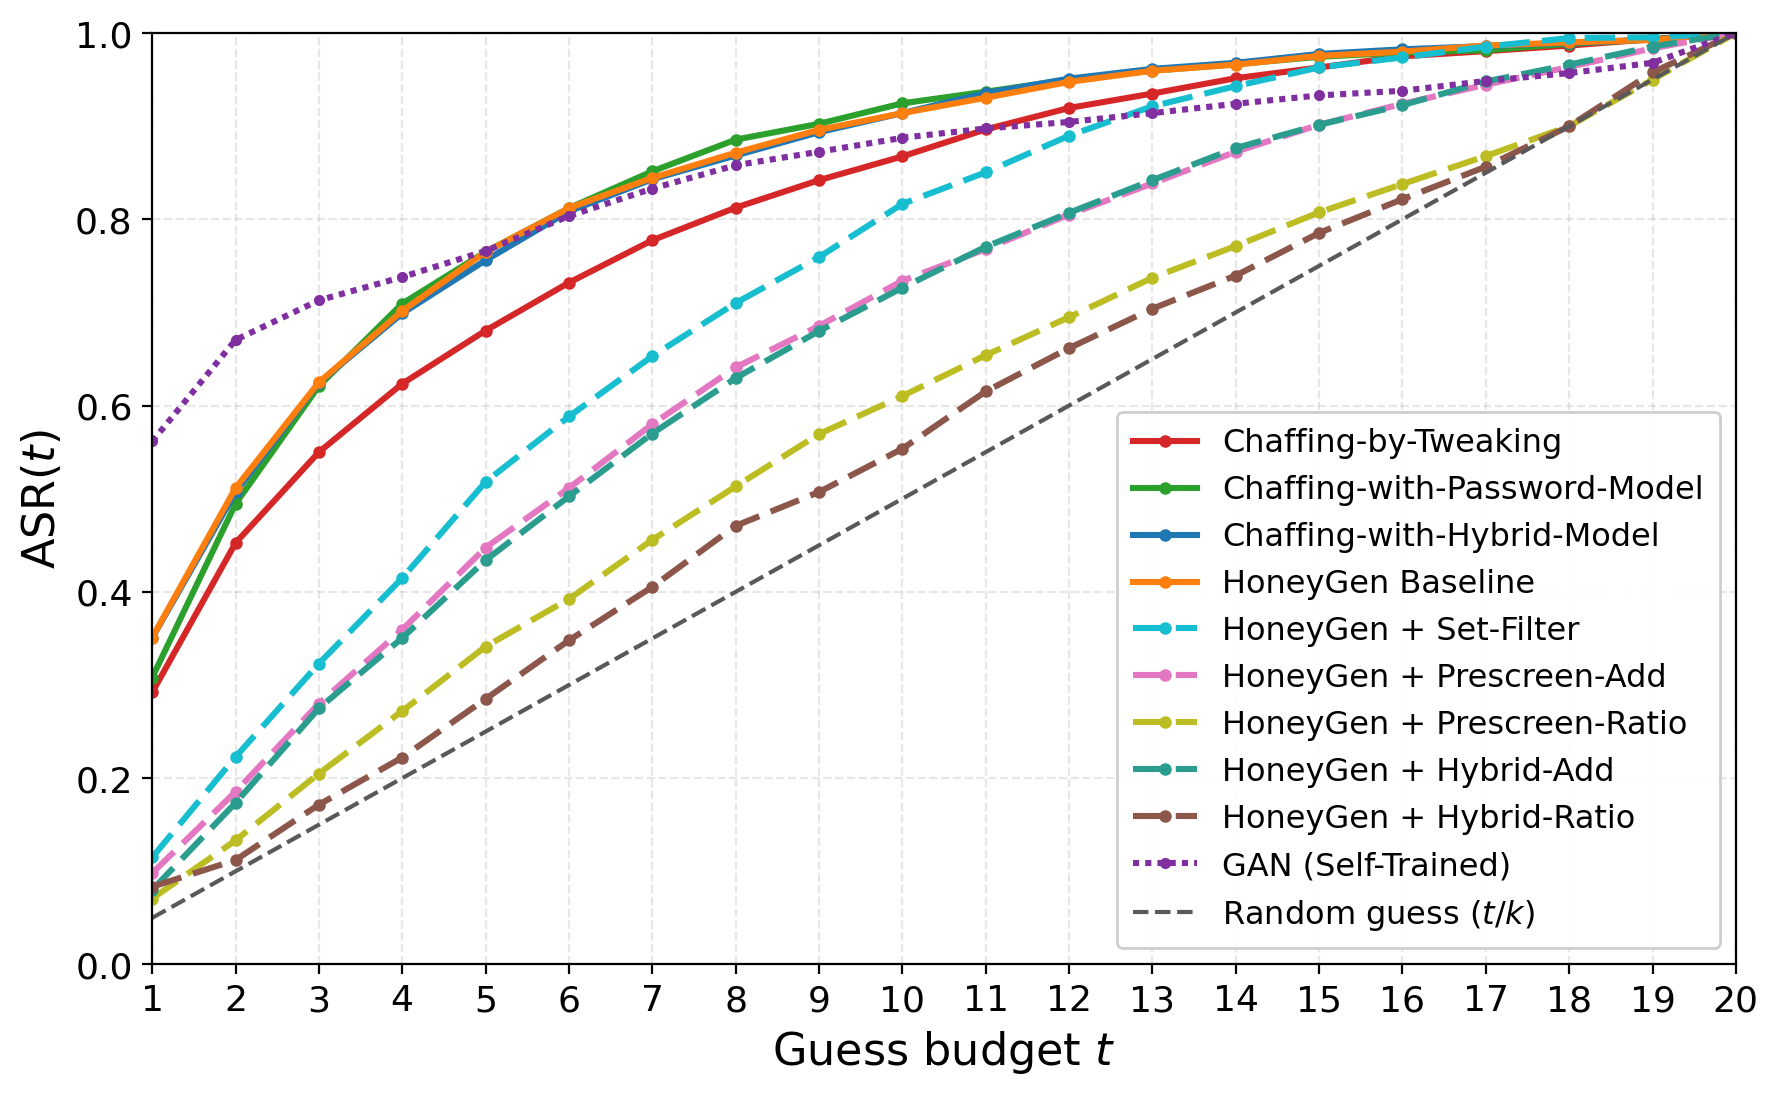
\includegraphics[width=\linewidth]{figures/cnn_N5000_e2000.png}
    \caption{$N_{\text{train}} = 5000$.}
  \end{subfigure}

  \medskip
  \begin{subfigure}{0.66\textwidth}
    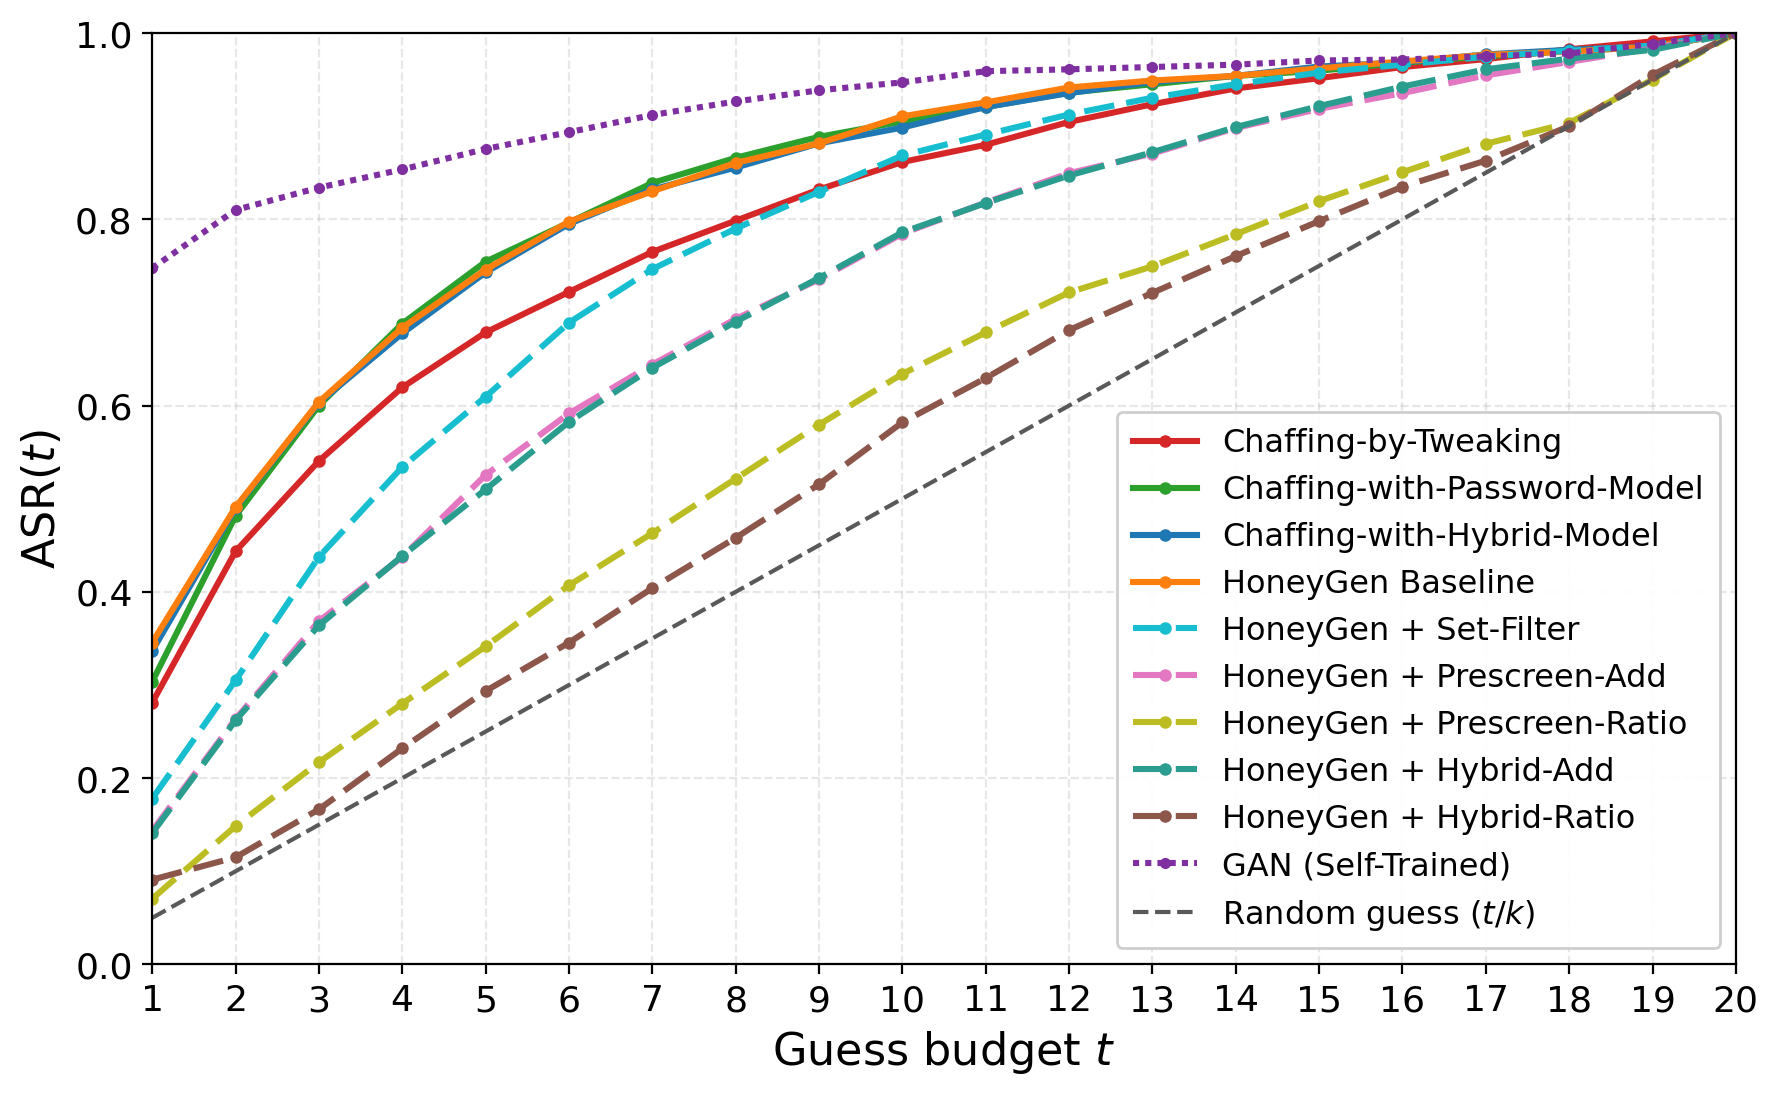
\includegraphics[width=\linewidth]{figures/cnn_N10000_e2000.png}
    \caption{$N_{\text{train}} = 10000$.}
  \end{subfigure}
  \caption{ASR curves under the CNN attacker for all ten methods, each
  evaluated on the same test set of 2000 sweetword sets, at the three
  training sizes. Curves report the rational-attacker value of
  \Cref{eq:rational}, so no method falls below the random-guessing
  diagonal. Solid lines are unfiltered generators, dashed lines are
  filtered variants, and the dotted line is the GAN.}
  \label{fig:cmp-all}
\end{figure}